\documentclass[11pt,a4paper]{article}

% ===== 纯黑白技术佐证报告 =====
\usepackage{fontspec}
\usepackage{xeCJK}
\setCJKmainfont[AutoFakeBold=2.5]{SimSun}
\setCJKsansfont[AutoFakeBold=2.5]{SimHei}
\setCJKmonofont{SimSun}
\setmainfont{Times New Roman}
\usepackage[margin=2.15cm,headheight=15pt]{geometry}
\usepackage{graphicx}
\usepackage{booktabs,array,tabularx}
\usepackage{xcolor}
\usepackage{enumitem}
\usepackage{fancyhdr}
\usepackage{caption}
\usepackage{hyperref}
\usepackage{tikz}
\usepackage{float}
\usepackage{amsmath}
\usetikzlibrary{positioning,arrows.meta,fit,calc}

\definecolor{ink}{RGB}{21,34,47}
\definecolor{grayink}{RGB}{93,103,112}
\definecolor{lightgray}{RGB}{238,240,242}
\definecolor{linegray}{RGB}{190,196,201}
\definecolor{white}{RGB}{255,255,255}
\hypersetup{hidelinks,pdftitle={Galen 技术佐证报告},pdfauthor={Galen Rehab Intelligence}}
\captionsetup{font=small,labelfont=bf,labelsep=quad}
\setlength{\parindent}{2em}
\setlength{\parskip}{0.25em}
\linespread{1.16}\selectfont
\newcolumntype{Y}{>{\raggedright\arraybackslash}X}
\newcommand{\Key}[1]{\textbf{#1}}
\newcommand{\Metric}[1]{{\fontsize{24}{27}\selectfont\bfseries #1}}
\newcommand{\Rule}{\par\noindent\rule{\linewidth}{0.45pt}\par}
\renewcommand{\contentsname}{目录}
\renewcommand{\figurename}{图}
\renewcommand{\tablename}{表}

\pagestyle{fancy}
\fancyhf{}
\lhead{\small\sffamily GALEN TECHNICAL EVIDENCE}
\rhead{\small\sffamily 技术佐证报告}
\cfoot{\small\thepage}
\renewcommand{\headrulewidth}{0.4pt}

\begin{document}

% ===== 封面 =====
\begin{titlepage}
\thispagestyle{empty}
\vspace*{1.8cm}
{\sffamily\large\bfseries GALEN REHAB INTELLIGENCE\par}
\vspace{0.22cm}
\rule{\linewidth}{1.1pt}\par
\vspace{1.2cm}
{\fontsize{28}{36}\selectfont\bfseries
面向康复科研的数据治理与\\
项目上下文执行引擎\par}
\vspace{0.55cm}
{\Large 技术佐证报告\par}
\vspace{1.4cm}
\noindent\begin{minipage}{0.88\linewidth}
\large
本报告回答一个具体问题：康复科研中的分散数据、反复沟通和不可追溯交付，能否被组织成一条可复核的执行链？我们以运动疲劳恢复为首个应用切口，将研究项目状态、脱敏 RehabID、外部工作台数据、工具调用和 LaTeX 论文交付放入同一条链路，并用自动化测试与真实运行产物验证其关键环节。
\end{minipage}

\vfill
\begin{tabularx}{\linewidth}{@{}lY@{}}
\toprule
报告版本 & v2.1 \\
验证日期 & 2026 年 9 月 13 日 \\
验证模型 & deepseek-v4-flash \\
验证对象 & Galen Context Engine 与 RehabID Connector 工作流 \\
\bottomrule
\end{tabularx}
\vspace{0.9cm}
\end{titlepage}

\section*{摘要}
\addcontentsline{toc}{section}{执行摘要}
康复科研中存在的瓶颈并不是缺少一个会回答问题的模型，而是数据与决定没有被组织成可持续使用的研究状态：量表、心率变异性（HRV）、动作表现、主观疲劳和治疗记录来自不同工具；研究范围会随着讨论修订；最终结果又常常停留在聊天文本中。研究者因此需要反复解释项目，难以判断某个结论来自哪份数据，也难以把一次分析复跑成正式交付物。

Galen 的解决方案是以项目为中心建立一层可更新的科研状态。PI 对话负责提出任务，Context Engine 维护当前问题、有效约束、排除范围、已确认事实与修订历史；Connector 把外部康复工作台的脱敏数据映射到 RehabID 和纵向时间轴；工具层负责检索、读取、写入和编译；每个关键判断都可以回到数据、证据或任务日志。换言之，Galen 不是把聊天记录做得更长，而是把“研究要什么、手里有什么、做过什么、为什么这样交付”变成系统对象。

本报告的验证范围是工程能力，不是临床疗效。我们验证了上下文能否持续、范围切换能否隔离、工具事实能否进入产物、RehabID 队列能否被导入，以及正式论文 PDF 能否由同一链路生成。结果为：上下文引擎自动化测试 40/40 通过；连续约束修订探针 9/9 通过；运动疲劳范围切换探针 8/8 通过；连接器流程形成可预览的 RehabID 队列和论文 PDF。基于这些结果，Galen 已从“聊天式助手原型”进入“康复科研数据治理与执行链原型”阶段。

\begin{center}
\begin{tabularx}{\linewidth}{@{}YYY@{}}
\toprule
\Metric{40/40} & \Metric{9/9} & \Metric{8/8} \\
上下文引擎自动化测试 & 连续约束修订探针 & 运动疲劳范围切换探针 \\
\bottomrule
\end{tabularx}
\end{center}

本次验证形成两组机器可读报告：其一检验三轮研究对话中的约束继承、工具读取事实保留与随访修订；其二检验从已归档方向切换至运动疲劳项目后，新方案仅使用当前协议、数据与变量。第二组测试在 33.000 秒内完成 8 项硬性断言，且旧方向关键词在正式方案与最终分析中均未出现。报告同时给出数据契约、指标定义、对照维度和未完成的外部验证，使评委能够区分“已经跑通的能力”和“下一步要证明的性能”。

在同一冻结任务卡上的受控框架对照中，Galen 75 次运行通过 72 次（96.0\%），Codex CLI 通过 17 次（22.7\%）；平均可观察工具调用为 1.96 对 11.64 次，中位总时延为 9.8 对 32.2 秒。该结果只说明在本协议定义的康复科研任务上，项目状态、数据契约和交付检查形成了可测的工程优势，不外推为对所有模型或所有临床任务的普遍结论。

\tableofcontents
\newpage

\section{问题定义：科研项目需要可控的状态}
研究对话通常面临两种相反的失败：同一项目中，系统要求研究者反复解释样本、结局和既有决定；项目范围已经变化时，系统又继续引用过时的病种、方法或方向。Galen 将这两个问题转化为项目状态管理问题。

\begin{figure}[htbp]
\centering
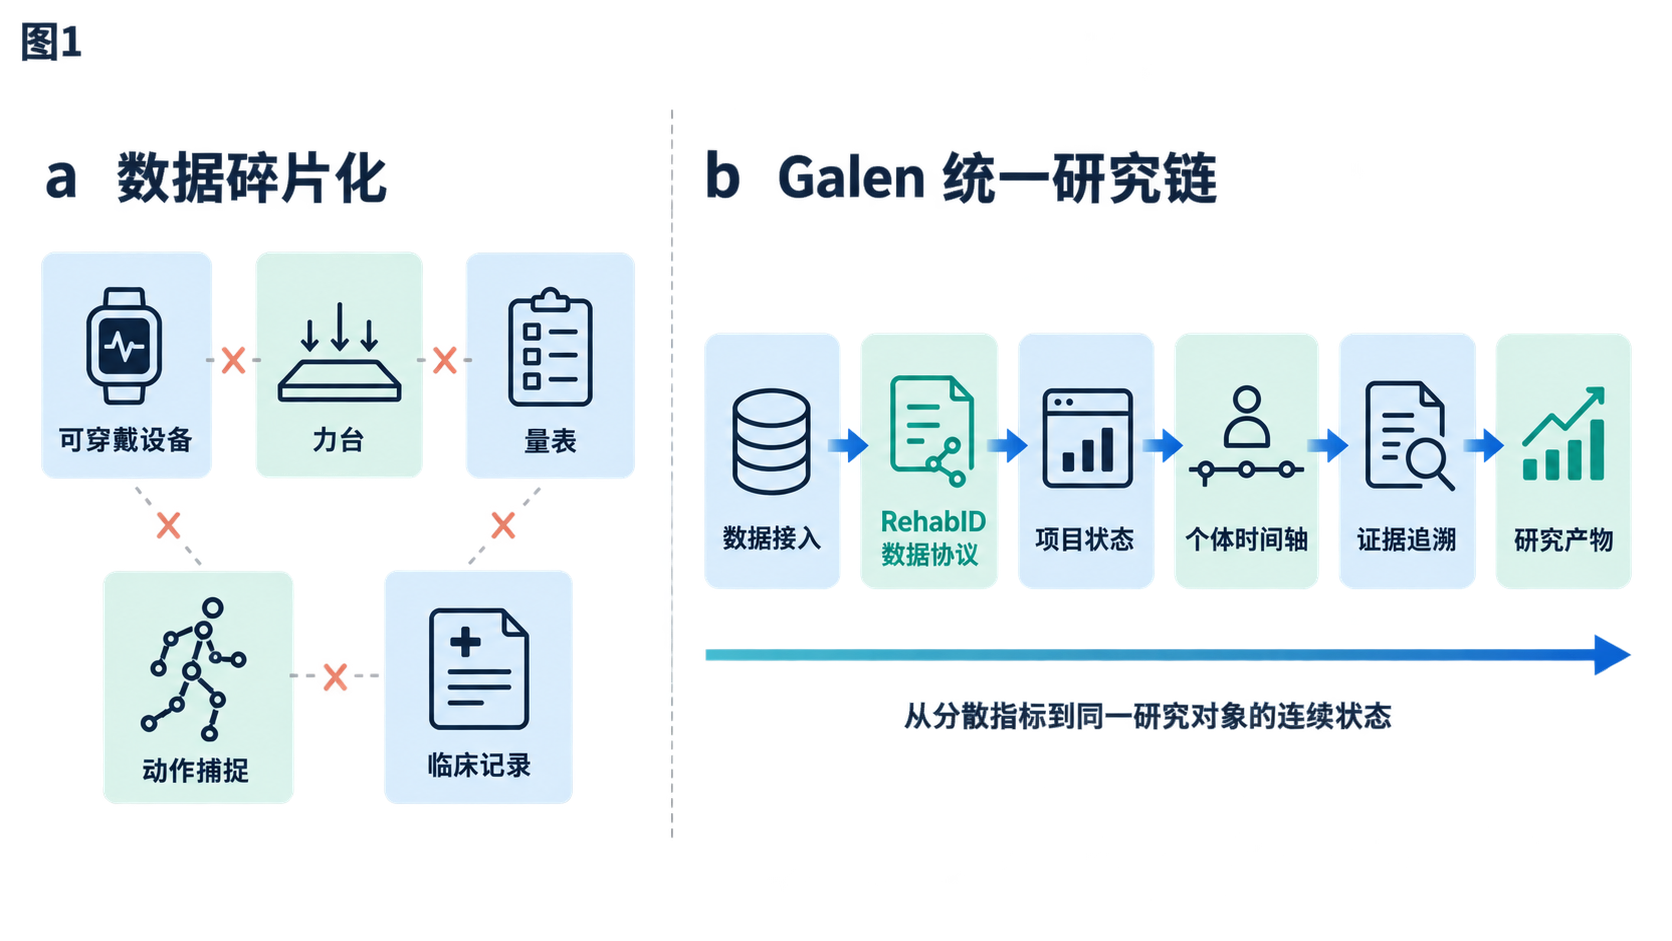
\includegraphics[width=0.98\linewidth]{assets/fig01-data-fragmentation-zh.png}
\caption*{从分散指标到同一研究对象的连续状态：Galen 将异构康复数据组织为统一、可追溯的研究链。}
\end{figure}

\subsection{要解决的不是“回答慢”，而是研究链断裂}
在运动疲劳研究中，一次完整的观察至少包含受试者身份、采集时间、任务阶段、HRV、动作表现、RPE/VAS、设备来源和质量标记。现实中这些信息通常分别存在于表格、设备导出文件、康复师工作台和聊天记录中。只要其中一个环节缺少时间或来源，研究者就无法可靠回答“变化发生在什么时候”“变化是否超过个人基线”“这个结论依据哪一条观察”。

因此，本项目将问题定义为三个可检验的工程命题：
\begin{enumerate}[leftmargin=2.1em,itemsep=3pt]
\item \textbf{状态连续性：}同一项目后续任务能否自动继承仍有效的协议、样本、变量和已确认事实，而不要求研究者重复输入；
\item \textbf{范围隔离：}研究方向发生切换后，旧病种、旧结局或旧假设能否退出当前推理，同时保留审计记录；
\item \textbf{交付可复核：}外部数据经过接入、清洗、对齐和分析后，能否形成带来源入口的正式研究产物，而不是一段无法复跑的聊天文字。
\end{enumerate}

\subsection{研究假设与验证边界}
我们的工程假设是：\textbf{显式的项目状态 + 统一的 RehabID 数据契约 + 可追溯的工具/产物链，比仅依赖聊天历史更适合承载连续科研任务。}若假设成立，则在相同任务下，系统应表现出更高的约束保留率、更低的范围泄漏率和更高的产物完成率。本报告只验证上述系统性质；尚未把这些性质等同于临床决策准确率，也没有声称 Galen 已完成多中心或前瞻性疗效验证。

\section{定位与创新：把科研上下文变成可计算对象}
\subsection{产品边界}
Galen 的首个应用切口是运动疲劳与恢复研究，但底层对象不绑定某个病种或设备。它面向的是康复科研的数据治理工作：把已有工作台、力台、可穿戴设备、量表和传感器数据纳入同一项目，并在研究问题变化时同步更新状态。硬件不是当前交付边界；当数据缺口被验证后，再决定是否设计专用传感器。

\subsection{相对于普通聊天与传统 RAG 的新增对象}
\begin{table}[H]
\centering
\small
\begin{tabularx}{\linewidth}{@{}p{2.9cm}YYY@{}}
\toprule
能力维度 & 普通聊天 & 传统文献检索/RAG & Galen 的项目化实现 \\
\midrule
上下文单位 & 当前会话 & 文档片段 & 具有版本和修订记录的 Project State \\
研究对象 & 文本中的称谓 & 文档中的实体 & 脱敏 RehabID 与纵向观察 \\
范围修订 & 依赖模型记忆 & 通常无显式排除范围 & active / archived / revised 三态管理 \\
数据接入 & 用户手动粘贴 & 以文本为主 & Connector 读取外部工作台并映射数据契约 \\
结论依据 & 隐含在回答中 & 片段级引用 & 数据、质量记录、文献和任务日志组成证据链 \\
交付形式 & 对话文本 & 摘要或引用列表 & 可预览、可下载、可复编译的 LaTeX/PDF 产物 \\
\bottomrule
\end{tabularx}
\caption{能力边界对照。表中“传统 RAG”是设计层面的参照，不代表本报告已完成外部框架的受控性能对比。}
\end{table}

\subsection{四项可复用的技术贡献}
\begin{enumerate}[leftmargin=2.1em,itemsep=4pt]
\item \textbf{项目状态模型：}把研究问题、当前范围、排除范围、协议约束、数据资产、证据来源、有效共识和修订历史作为结构化字段，而不是散落在 prompt 中；
\item \textbf{RehabID 数据契约：}用脱敏身份连接多次访视，保留时间、模态、变量、单位、质量状态和来源，使 HRV、CMJ、RPE/VAS 等观察可以在同一时间轴比较；
\item \textbf{工具—产物闭环：}研究任务可以调用检索、读取、写入、引用核验和 PDF/LaTeX 编译工具，工具结果进入项目状态并成为最终产物的一部分；
\item \textbf{可追溯交付：}从一条观察或一条文献到图表、结论和 PDF 页面保留反向入口，研究者可以验证“这句话从哪里来”，也可以复跑同一任务。
\end{enumerate}

\section{Galen 上下文工程架构设计}
Galen 的上下文工程不把“历史聊天记录越长越好”作为目标，而是围绕一个研究项目持续维护五类可计算对象：\textbf{项目上下文}定义研究问题、当前范围和排除范围；\textbf{数据上下文}组织 RehabID、时间点、变量、单位和质量标记；\textbf{证据上下文}保存文献、数据来源、覆盖状态和引用指针；\textbf{执行上下文}记录任务节点、工具调用、预算和中间产物；\textbf{交互上下文}保留研究者确认过的决定与必要的对话摘要。PI 对话负责提出和编排任务，Context Engine 负责选择、更新和审计这些对象。

\begin{figure}[H]
\centering
\begin{tikzpicture}[font=\small, node distance=0.55cm and 0.52cm,
  box/.style={draw=ink, rounded corners=2pt, minimum height=1.05cm, align=center, fill=lightgray, text width=2.55cm},
  core/.style={draw=ink, line width=0.7pt, rounded corners=2pt, minimum height=1.3cm, align=center, fill=white, text width=3.05cm},
  output/.style={draw=ink, rounded corners=2pt, minimum height=0.9cm, align=center, fill=white, text width=2.6cm},
  flow/.style={-{Latex[length=2.1mm]}, line width=0.65pt, draw=ink}]
  \node[box] (project) {项目上下文\\研究问题 / 有效范围 / 排除范围};
  \node[box, below=of project] (data) {数据上下文\\RehabID / 时间轴 / 质量标记};
  \node[box, below=of data] (evidence) {证据上下文\\来源 / 覆盖状态 / 引用指针};
  \node[box, below=of evidence] (execution) {执行上下文\\任务节点 / 工具轨迹 / 产物};
  \node[box, below=of execution] (interaction) {交互上下文\\确认决定 / 对话摘要 / 修订记录};
  \node[core, right=1.05cm of data.south east, yshift=0.82cm] (engine) {Galen\\Context Engine\\选择当前有效状态\\拼装任务上下文\\写入修订与审计轨迹};
  \node[output, right=1.05cm of engine] (pi) {PI 对话\\提出问题与确认决策};
  \node[output, below=0.52cm of pi] (tools) {工具层\\检索 / 分析 / 编译};
  \node[output, below=0.52cm of tools] (artifact) {研究产物\\证据链 / 图表 / PDF};
  \draw[flow] (project.east) -- (engine.west |- project.east);
  \draw[flow] (data.east) -- (engine.west |- data.east);
  \draw[flow] (evidence.east) -- (engine.west |- evidence.east);
  \draw[flow] (execution.east) -- (engine.west |- execution.east);
  \draw[flow] (interaction.east) -- (engine.west |- interaction.east);
  \draw[flow] (engine.east) -- (pi.west);
  \draw[flow] (pi.south) -- (tools.north);
  \draw[flow] (tools.south) -- (artifact.north);
  \draw[flow] (artifact.west) -| ([xshift=0.42cm]engine.south) |- (engine.south);
\end{tikzpicture}
\caption{Galen 上下文工程架构。上下文不再是单一 prompt，而是项目、数据、证据、执行和交互五类状态的协同系统。}
\label{fig:context-engineering}
\end{figure}

\subsection{上下文选择与状态更新规则}
每次任务开始前，Context Engine 先读取当前项目状态 $S_t$，再根据任务意图 $I_t$ 选取最小充分上下文，而非无差别拼接全部历史：
\[
C_t=\operatorname{Compose}(S_t, D_t, R_t, X_t \mid I_t),
\]
其中 $D_t$ 为已纳入项目的数据资产，$R_t$ 为可用证据，$X_t$ 为可执行任务与工具状态。选择过程遵守三条规则：\textbf{有效优先}，仅注入 active 状态的范围和决策；\textbf{任务相关}，仅取与当前分析、检索或交付直接相关的数据切片；\textbf{历史可审计}，已归档或被修订内容不进入当前推理，但保留其版本和替换关系。

当研究者修改范围、确认新的事实或导入新数据时，系统不是简单在聊天末尾追加一句文本，而是写入有来源、有时间戳的状态事件 $e_t$：
\[
S_{t+1}=\operatorname{Apply}(S_t,e_t),\qquad H_{t+1}=H_t\cup\{e_t\}.
\]
这里 $S_{t+1}$ 进入下一次推理，$H_{t+1}$ 形成可回看的修订轨迹。因此，同一机制同时解决“该记住的约束被保留”和“已经退出的方向不再干扰当前任务”两个问题。

\subsection{架构单元与可验证证据}
\begin{table}[H]
\centering
\small
\begin{tabularx}{\linewidth}{@{}p{3.0cm}Yp{3.1cm}@{}}
\toprule
架构单元 & 工程行为 & 本轮可核验证据 \\
\midrule
项目状态与有效范围 & 将当前研究范围、排除方向和确认决定写成可更新字段；修订后仅使有效条目进入后续任务 & 运动疲劳项目接管探针 8/8 通过；旧方向未进入新方案 \\
约束继承与任务摘要 & 从协议、样本、结局和工具事实中选取当前任务所需约束，并随任务节点持续继承 & 三轮连续约束修订探针 9/9 通过 \\
数据与证据上下文 & 将 RehabID 队列、时间点、变量、质量标记和来源指针绑定到研究项目 & 连接器导入形成 12 个 RehabID、48 个时间点与 204 条观察记录 \\
执行与产物上下文 & 记录工具调用、分析步骤和 LaTeX/PDF 产物，供下一节点读取和回溯 & 上下文引擎自动化测试 40/40 通过；正式 PDF 已交付 \\
\bottomrule
\end{tabularx}
\caption{上下文工程架构从抽象设计到可执行验证的对应关系。}
\label{tab:context-engineering-evidence}
\end{table}

\section{核心机制：有效约束进入下一轮推理}
项目状态由七类信息组成：研究问题、当前范围、排除范围、数据资产、证据来源、有效共识与修订历史。研究者修订决策后，新决策替代旧决策；只有有效条目进入后续任务的上下文，历史条目保留在审计轨迹中。

\begin{figure}[htbp]
\centering
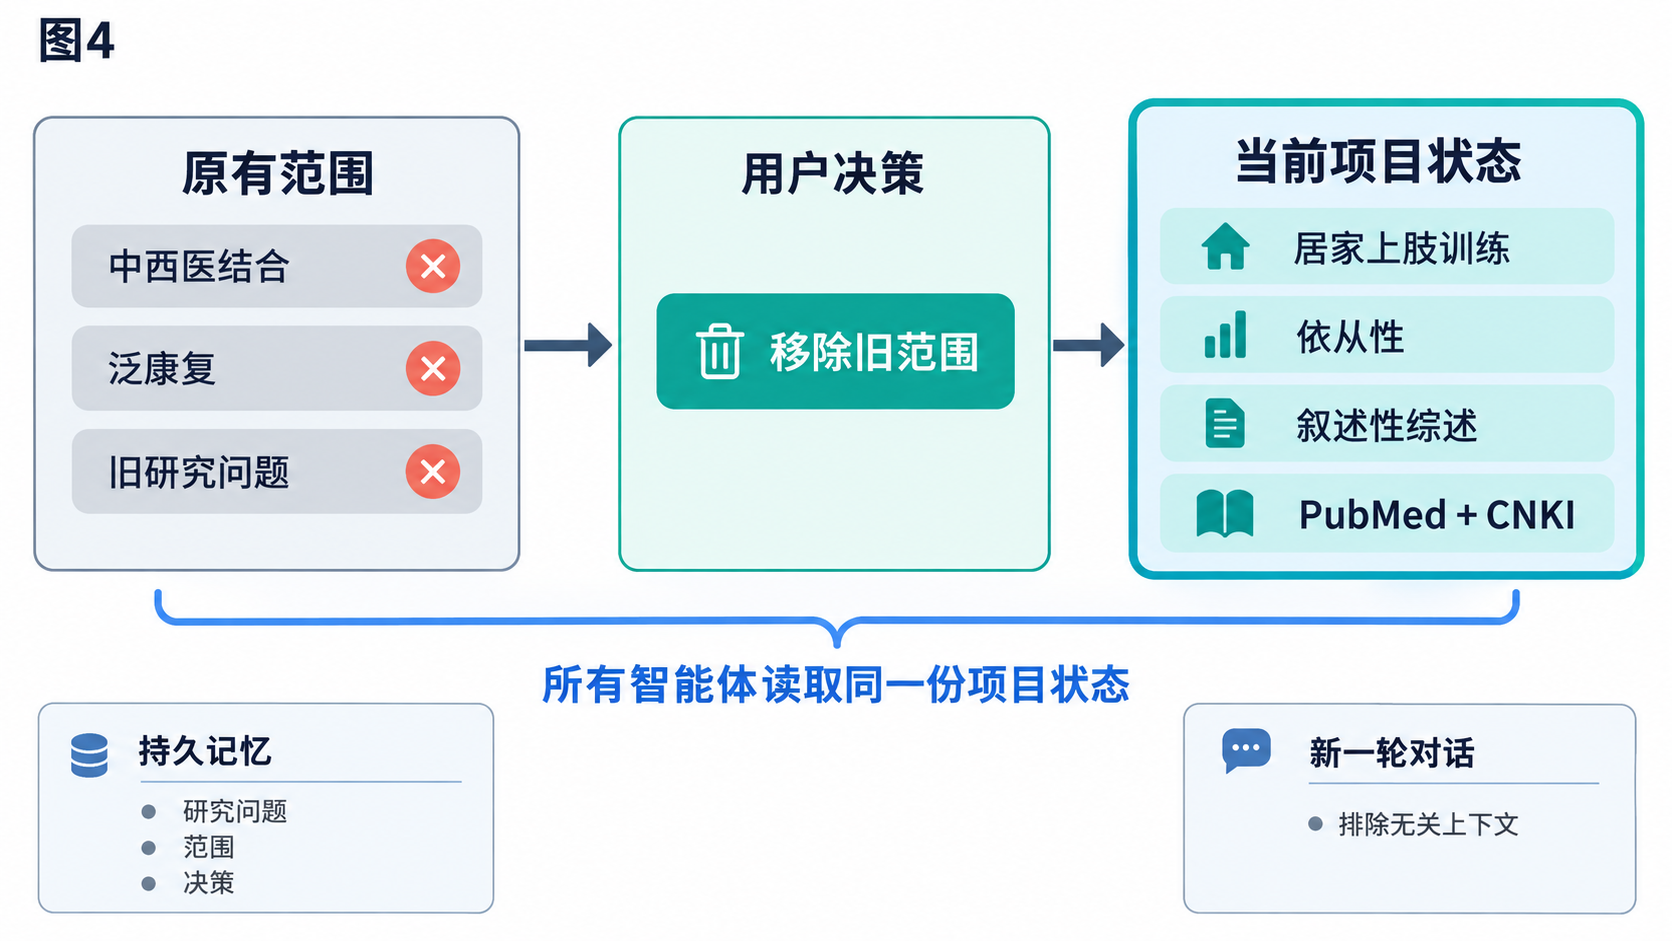
\includegraphics[width=0.98\linewidth]{assets/fig04-project-state-zh.png}
\caption*{范围切换规则：历史可追溯，当前任务只服从有效项目状态。}
\end{figure}

\section{系统实现：从接入到交付的六步链路}
Galen 的运行链不是“提问—生成”两步，而是一个可以检查中间状态的六步过程。每一步都有输入、处理和可观察产物，便于定位错误，也便于把一次演示转化为可重复的研究任务。

\begin{table}[H]
\centering
\small
\begin{tabularx}{\linewidth}{@{}c p{3.1cm} Y Y@{}}
\toprule
步骤 & 处理环节 & 关键操作 & 可观察产物 \\
\midrule
1 & 接入（Ingest） & Connector 发现外部工作台的脱敏队列和数据源 & RehabID 列表、来源标识 \\
2 & 规范化（Normalize） & 将 CSV/JSON/量表/设备记录映射到统一字段 & 变量名、单位和时间格式 \\
3 & 质检（QC） & 检查缺失、重复、异常值和时间顺序 & 每条观察的质量状态与问题清单 \\
4 & 对齐（Align） & 按 RehabID、访视和任务阶段组织纵向数据 & 个体时间轴、队列矩阵 \\
5 & 推理（Reason） & PI 对话调用分析、检索和引用工具，读取当前项目状态 & 分析结果、证据指针、修订日志 \\
6 & 交付（Deliver） & 将图表、方法、结果和引用编译为正式 PDF & LaTeX 源码、PDF、预览链接 \\
\bottomrule
\end{tabularx}
\caption{Galen 的端到端科研执行链。}
\end{table}

\subsection{核心数据契约}
RehabID 不是设备编号，也不是患者姓名，而是研究范围内的脱敏数据身份。最小观察记录可以表示为：
\[
o_i=\langle r_i, t_i, m_i, v_i, x_i, u_i, q_i, p_i\rangle,
\]
其中 $r_i$ 为 RehabID，$t_i$ 为采集时间或访视，$m_i$ 为数据模态，$v_i$ 为变量名，$x_i$ 为数值或结构化值，$u_i$ 为单位，$q_i$ 为质量状态，$p_i$ 为来源指针。这个契约让“HRV 下降”不再是无来源的一句话，而是可以定位到某个个体、某个时间点、某个设备导出和对应的质检记录。

项目状态则维护为：
\[
S_t=\{Q_t,A_t,E_t,D_t,R_t,H_t\},
\]
其中 $Q_t$ 是研究问题，$A_t$ 是当前有效范围，$E_t$ 是排除范围，$D_t$ 是数据资产，$R_t$ 是证据与来源，$H_t$ 是修订历史。新任务读取 $S_t$；修订只更新有效字段，不删除审计记录。这是 Galen 能够“该记住时记住、该忘记时退出”的实现基础。

\subsection{运动疲劳首个示例}
本项目以一个可复跑的脱敏队列作为演示切口：12 名研究对象、48 个时间点，围绕 HRV、CMJ、RPE/VAS 和 72 小时观察窗组织数据。系统的任务不是给出一个脱离上下文的“疲劳/不疲劳”标签，而是将多时间点变化与个人基线、任务阶段和数据质量一起呈现，支持研究者进一步检验恢复轨迹、指标之间的关系和干预反应。该队列用于验证数据链路与科研交付，不在本报告中推导人群疗效结论。

\section{可执行验证一：三轮连续约束修订}
\subsection{测试设计}
连续约束修订探针以三轮真实模型调用完成：第一轮建立研究协议号、样本量、主要结局和 12 周随访；第二轮读取资格标准文件并写入研究方案；第三轮将随访由 12 周修订为 16 周，同时验证模型是否仍保留第一轮协议约束与第二轮工具读取的证据代码。

\begin{table}[htbp]
\centering
\small
\begin{tabularx}{\linewidth}{@{}cY Y@{}}
\toprule
轮次 & 系统动作 & 验收重点 \\
\midrule
1 & 建立协议 GALEN-CONTEXT-73 与核心约束 & 首次信息成为后续项目状态 \\
2 & 读取资格标准并写入 \texttt{context-protocol.md} & 工具读取事实进入方案产物 \\
3 & 修订随访 12 周至 16 周并进行方案复盘 & 保留有效事实，应用最新修订 \\
\bottomrule
\end{tabularx}
\caption{连续约束修订探针的三轮任务。}
\end{table}

\subsection{真实运行结果}
\begin{center}
\begin{tabularx}{\linewidth}{@{}Yccc@{}}
\toprule
验证项目 & 结果 & 数值 & 证据 \\
\midrule
轮次历史继承 & 通过 & 2 条 / 5 条历史消息 & 第 2、3 轮分别读取前序交换 \\
工具调用 & 通过 & \texttt{read\_file} + \texttt{write\_file} & 研究方案真实写入 \\
初始约束保留 & 通过 & 4 项核心约束 & 协议、样本、结局、旧随访均被识别 \\
修订应用 & 通过 & 12 周 $\rightarrow$ 16 周 & 最新随访被应用 \\
工具事实保留 & 通过 & 资格标准 + E-TOOL-29 & 第 2 轮读取事实在第 3 轮可用 \\
总判定 & \textbf{通过} & \textbf{9/9} & 55.998 秒 \\
\bottomrule
\end{tabularx}
\end{center}

\section{可执行验证二：旧方向退出与运动疲劳项目接管}
\subsection{测试设计}
本测试直接对应 Galen 的核心产品承诺。第一轮保留已归档的历史方向；第二轮正式切换至运动疲劳恢复项目 \texttt{GALEN-FATIGUE-01}，读取数据字典并生成新方案；第三轮在不重复研究范围、不调用工具的情况下，要求系统给出 HRV、CMJ 和 RPE 的纵向分析方案。验收要求为：当前项目约束完整保留，归档方向不得出现在新方案或最终回答。

\begin{figure}[htbp]
\centering
\begin{tikzpicture}[
  every node/.style={font=\small},
  stage/.style={draw=ink,rounded corners=3pt,minimum width=4.15cm,minimum height=1.45cm,align=left,fill=white},
  arrow/.style={-{Stealth[length=2.5mm]},thick,draw=ink}
]
\node[stage] (a) {\textbf{01 历史项目}\\[-1mm]已有讨论进入审计轨迹};
\node[stage,right=0.8cm of a] (b) {\textbf{02 范围切换}\\[-1mm]GALEN-FATIGUE-01 成为当前范围};
\node[stage,right=0.8cm of b] (c) {\textbf{03 新任务交付}\\[-1mm]生成运动疲劳方案与纵向分析};
\draw[arrow] (a)--(b);
\draw[arrow] (b)--(c);
\node[below=0.35cm of b,text=grayink] {当前数据：12 名受试者、48 时点、HRV / CMJ / RPE、72 小时};
\end{tikzpicture}
\caption{运动疲劳项目接管的范围控制流程。}
\end{figure}

\begin{table}[htbp]
\centering
\small
\begin{tabularx}{\linewidth}{@{}YccY@{}}
\toprule
硬性断言 & 结果 & 数值 & 验证内容 \\
\midrule
前序对话继承 & 通过 & 2 / 5 条历史消息 & 三轮会话持久化 \\
数据字典读写 & 通过 & 2 个工具动作 & 读取数据字典并写入新方案 \\
当前项目约束保留 & 通过 & 8 项字段 & 协议、样本、时点、变量、证据代码完整出现 \\
归档方向泄漏 & 通过 & 0 个关键词 & 正式方案与最终回答均未出现归档方向 \\
最终交付完整性 & 通过 & 1 份方案 + 1 段分析 & 结尾与内容结构完整 \\
总判定 & \textbf{通过} & \textbf{8/8，33.000 秒} & 完整通过 \\
\bottomrule
\end{tabularx}
\caption{运动疲劳范围切换探针的真实运行结果。}
\end{table}

\begin{figure}[htbp]
\centering
\begin{tikzpicture}[x=1cm,y=0.42cm,font=\small]
\draw[->,thick] (0,0) -- (13,0) node[right] {通过断言数};
\foreach \x/\lab in {0/0,3/3,6/6,9/9} {\draw (\x,0.12)--(\x,-0.12) node[below] {\lab};}
\fill[ink] (0,1.1) rectangle (9,1.95);
\node[right] at (9.2,1.52) {连续约束修订：9 / 9};
\fill[grayink] (0,3.15) rectangle (8,4.0);
\node[right] at (8.2,3.57) {运动疲劳范围切换：8 / 8};
\end{tikzpicture}
\caption{两组真实上下文探针的硬性断言通过数。}
\end{figure}

\section{评测体系：把“好用”拆成可测指标}
为了避免只展示漂亮界面，本项目把验收拆为五类指标。每类指标都对应一个可以在日志、产物或人工复核中找到的证据。

\begin{table}[H]
\centering
\small
\begin{tabularx}{\linewidth}{@{}p{3.1cm}p{3.5cm}Y@{}}
\toprule
指标 & 定义 & 本轮证据与解释 \\
\midrule
约束保留率 $R$ & 后续任务仍正确保留的必需约束数 / 必需约束总数 & 连续探针中协议、样本、结局和修订字段均被识别；对应断言通过 \\
范围隔离率 $S$ & $1-$（泄漏的归档条目数 / 归档条目检查数） & 运动疲劳探针旧方向关键词泄漏为 0，故 $S=1.00$（在本测试集上） \\
工具完成率 $T$ & 已生成的必需产物数 / 任务要求的产物数 & 真实调用完成读取资格标准、写入方案和 PDF 交付 \\
产物有效率 $V$ & 可打开且结构完整的产物数 / 生成产物总数 & 两组 JSON、方案文件和 PDF 均可读取；PDF 通过页面级渲染检查 \\
证据覆盖率 $C$ & 带数据/文献/日志来源指针的关键主张数 / 需要来源的关键主张总数 & 当前已实现来源链和预览入口；逐条主张统计仍列为下一轮人工审计 \\
\bottomrule
\end{tabularx}
\caption{Galen 当前的核心评测指标。公式用于统一后续对照实验口径。}
\end{table}

\subsection{本轮运行开销}
机器可读报告还记录了模型调用的输入/输出令牌和总耗时，作为后续比较工具调用经济性的基线，而不是未经对照的“优于其他框架”结论：连续约束修订探针使用 25,217 个输入令牌和 8,264 个输出令牌，总耗时 55.998 秒；运动疲劳范围切换探针使用 18,433 个输入令牌和 4,529 个输出令牌，总耗时 33.000 秒。下一阶段将用相同任务卡、相同模型和相同数据，和无项目状态的基线系统进行配对实验，比较 $R$、$S$、$T$、$C$ 及令牌开销。

\subsection{为什么先做工程指标}
如果上下文、数据和来源都不稳定，任何临床预测准确率都无法解释：模型可能只是记住了上一轮文本，或者在缺少时间和质量标记的情况下拼接出看似合理的结论。因此当前阶段先验证“数据是否进入了正确的项目、状态是否按修订更新、产物是否可以复核”，再开展统计效能、跨设备泛化和临床相关性研究。这样的顺序让每个后续结果都能追溯到一条可靠的数据链。

\newpage
\section{RehabID 连接器：将外部工作数据带入研究状态}
连接器不是页面跳转，而是将外部康复工作台中的脱敏数据作为 Galen 可调用的数据插件。研究者在工作台完成日常接诊、评估与报告；需要科研分析时，Galen 通过连接器提取已选择的 RehabID 队列，并将数据纳入当前研究时间轴。

\begin{figure}[htbp]
\centering
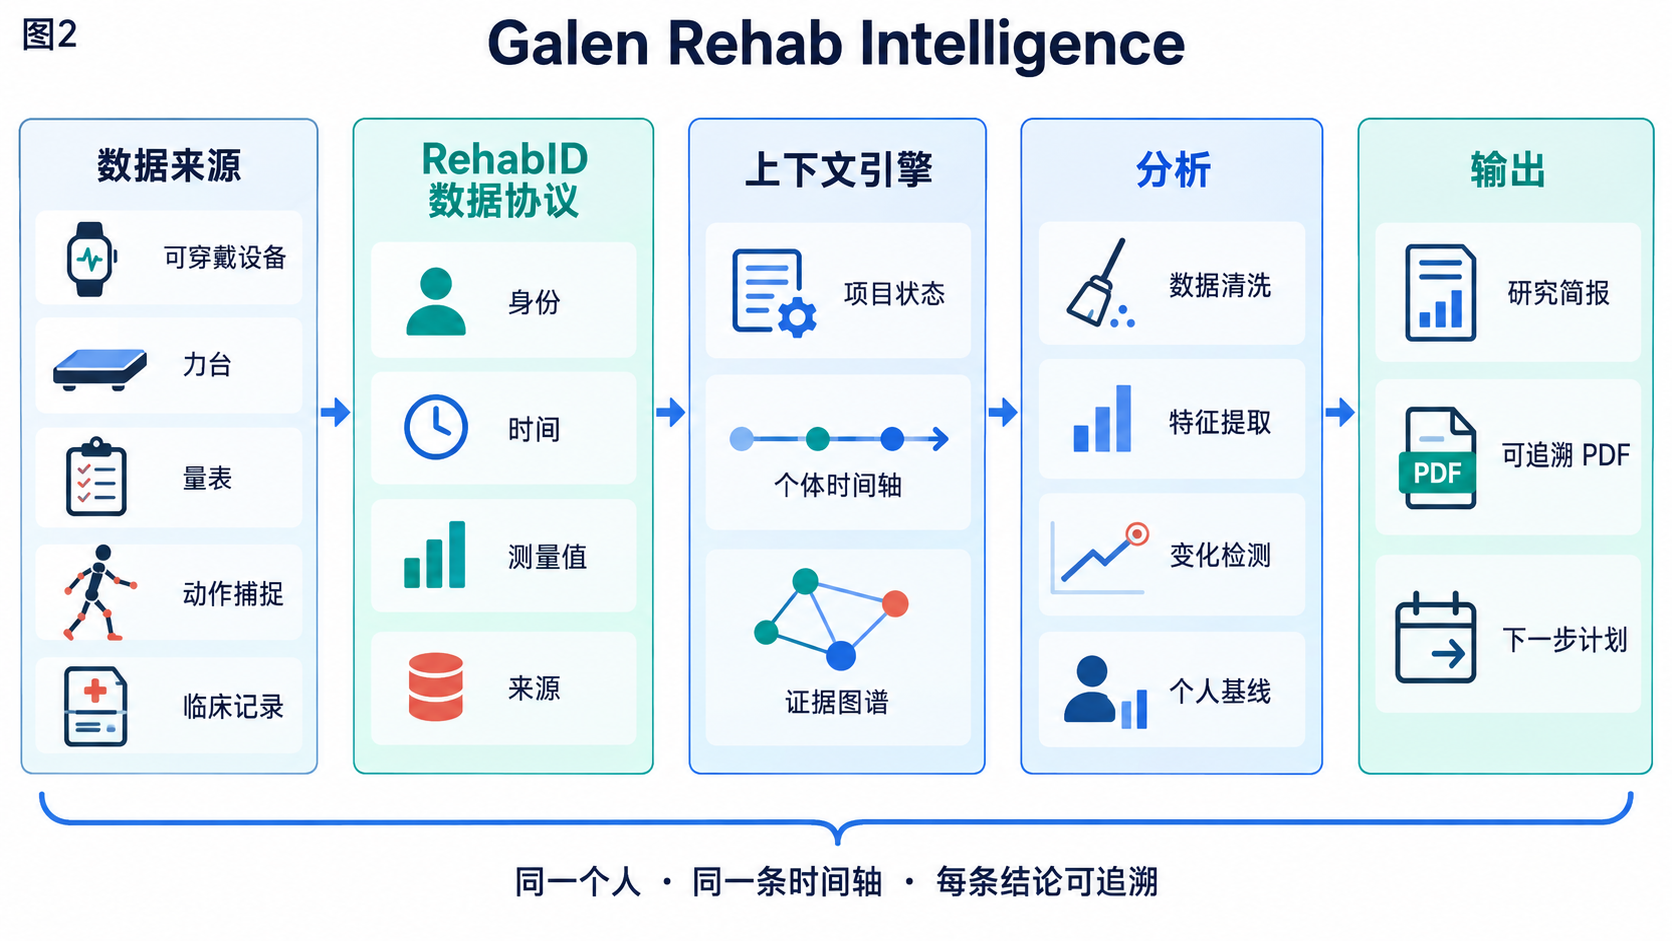
\includegraphics[width=0.98\linewidth]{assets/fig02-galen-architecture-zh.png}
\caption*{Galen 的五层架构：数据来源经 RehabID 数据协议和上下文引擎进入分析，最终形成可追溯科研产物。}
\end{figure}

\begin{figure}[htbp]
\centering
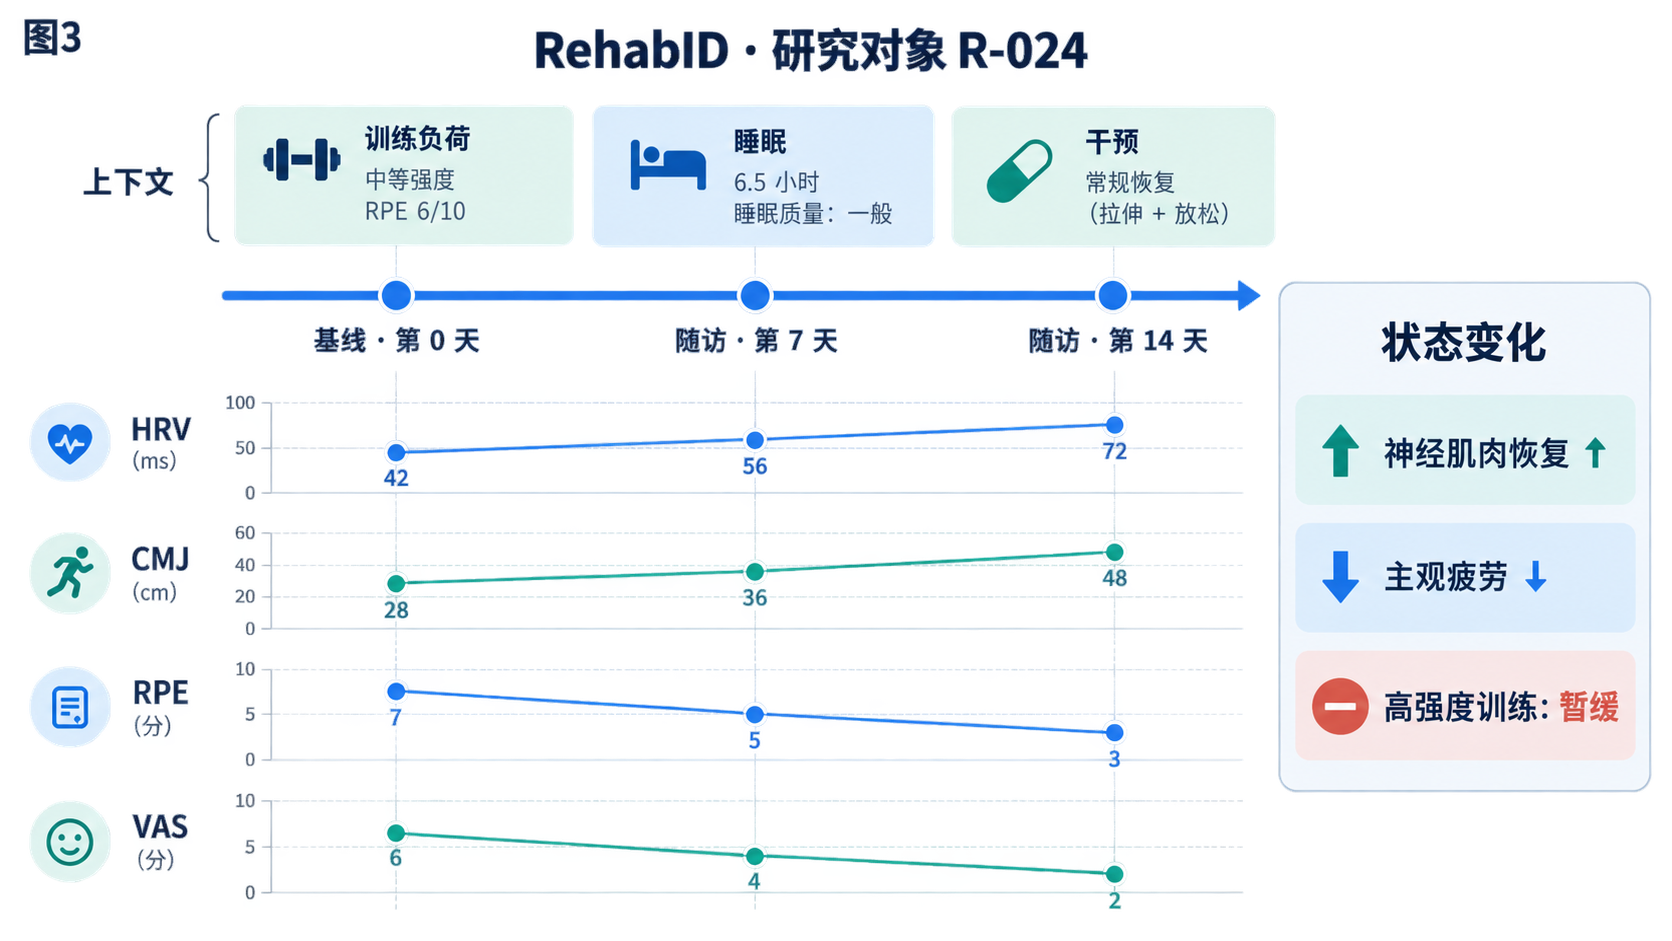
\includegraphics[width=0.98\linewidth]{assets/fig03-rehabid-timeline-zh.png}
\caption*{同一研究对象的纵向时间轴：HRV、CMJ、RPE 与 VAS 在同一 RehabID 上按访视对齐。}
\end{figure}

\begin{figure}[htbp]
\centering
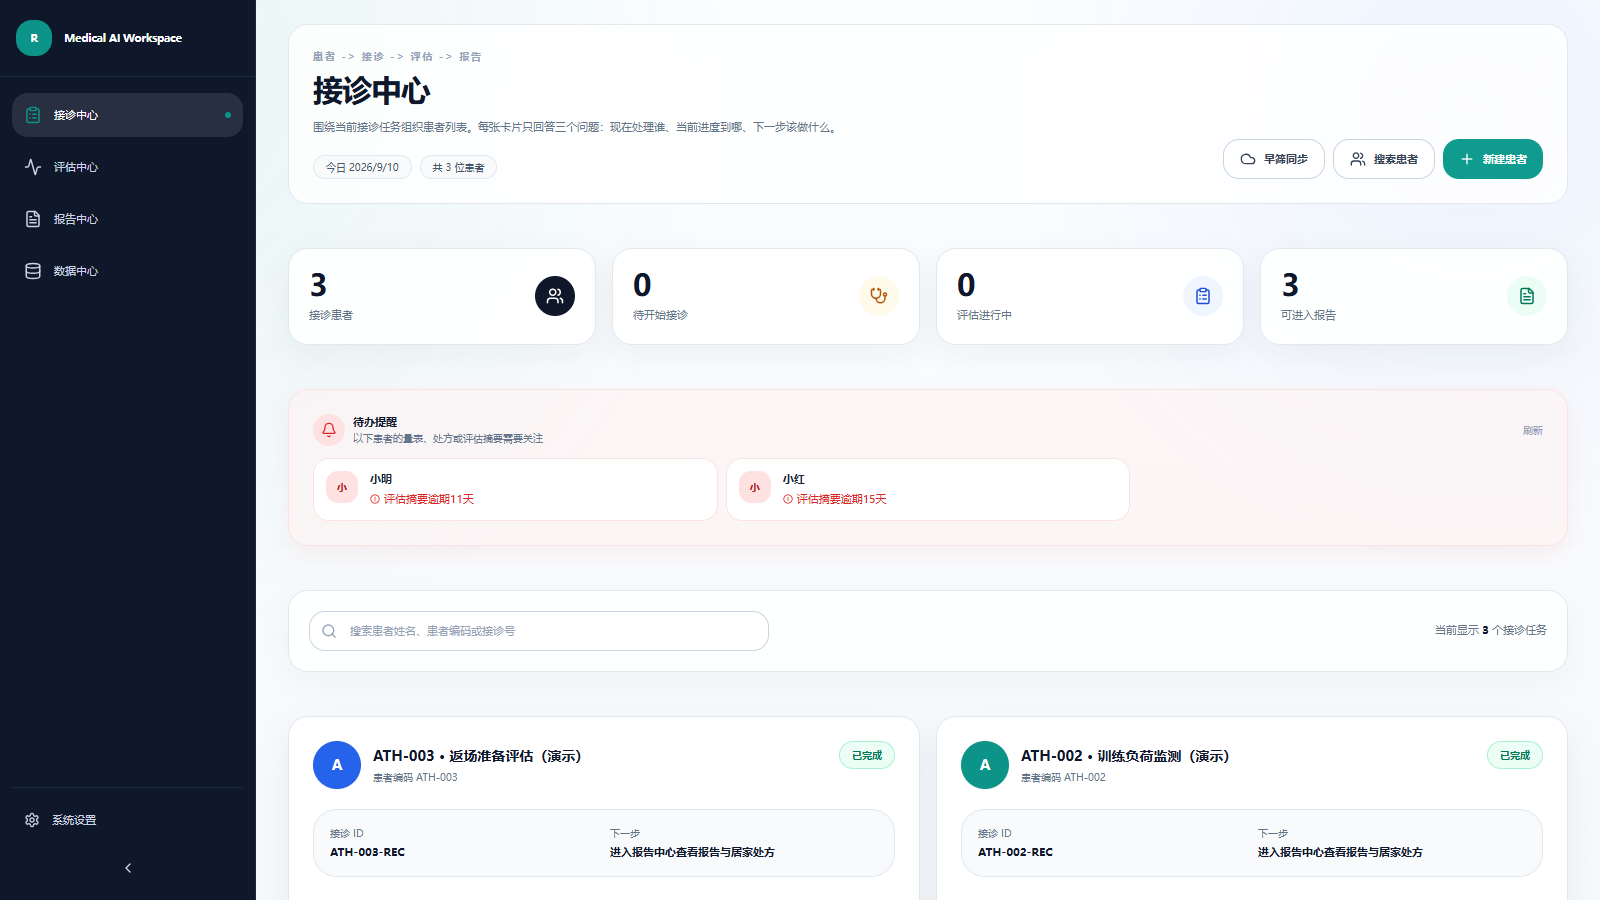
\includegraphics[width=0.94\linewidth]{assets/rehab-workbench.png}
\caption{康复师工作台中的接诊与评估任务。图中为脱敏演示队列。}
\end{figure}

\begin{figure}[htbp]
\centering
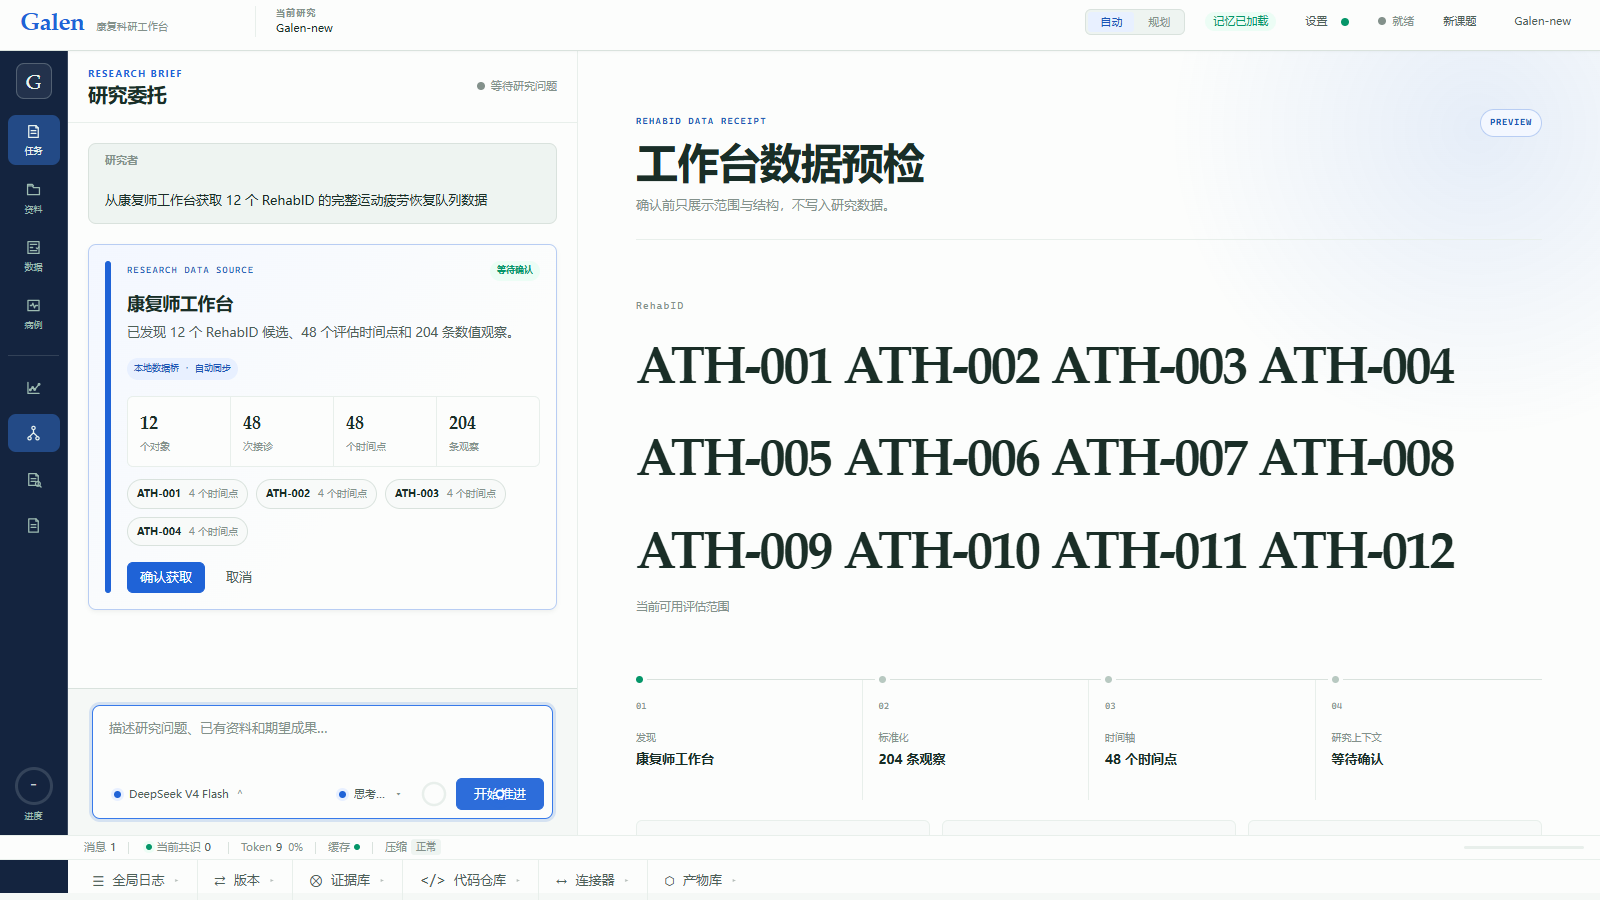
\includegraphics[width=0.94\linewidth]{assets/connector-preview.png}
\caption{Galen 连接器发现 12 个 RehabID、48 个评估时点及 204 条核心观察。}
\end{figure}

\begin{figure}[htbp]
\centering
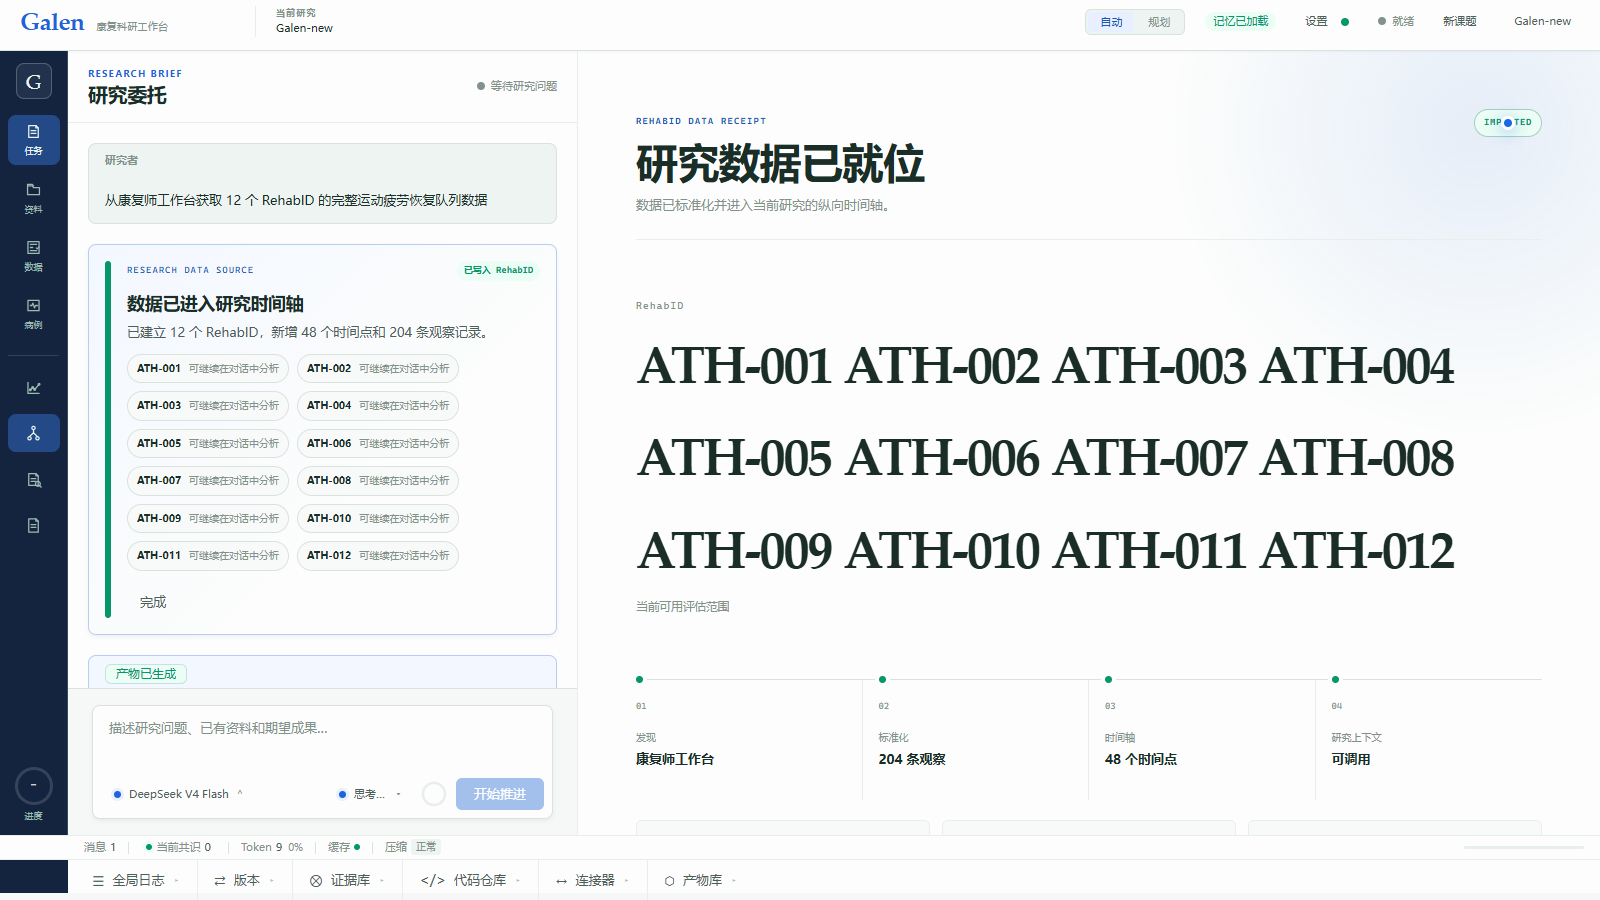
\includegraphics[width=0.94\linewidth]{assets/rehabid-imported.png}
\caption{确认导入后，RehabID 队列进入当前研究的纵向时间轴。}
\end{figure}

\begin{figure}[htbp]
\centering
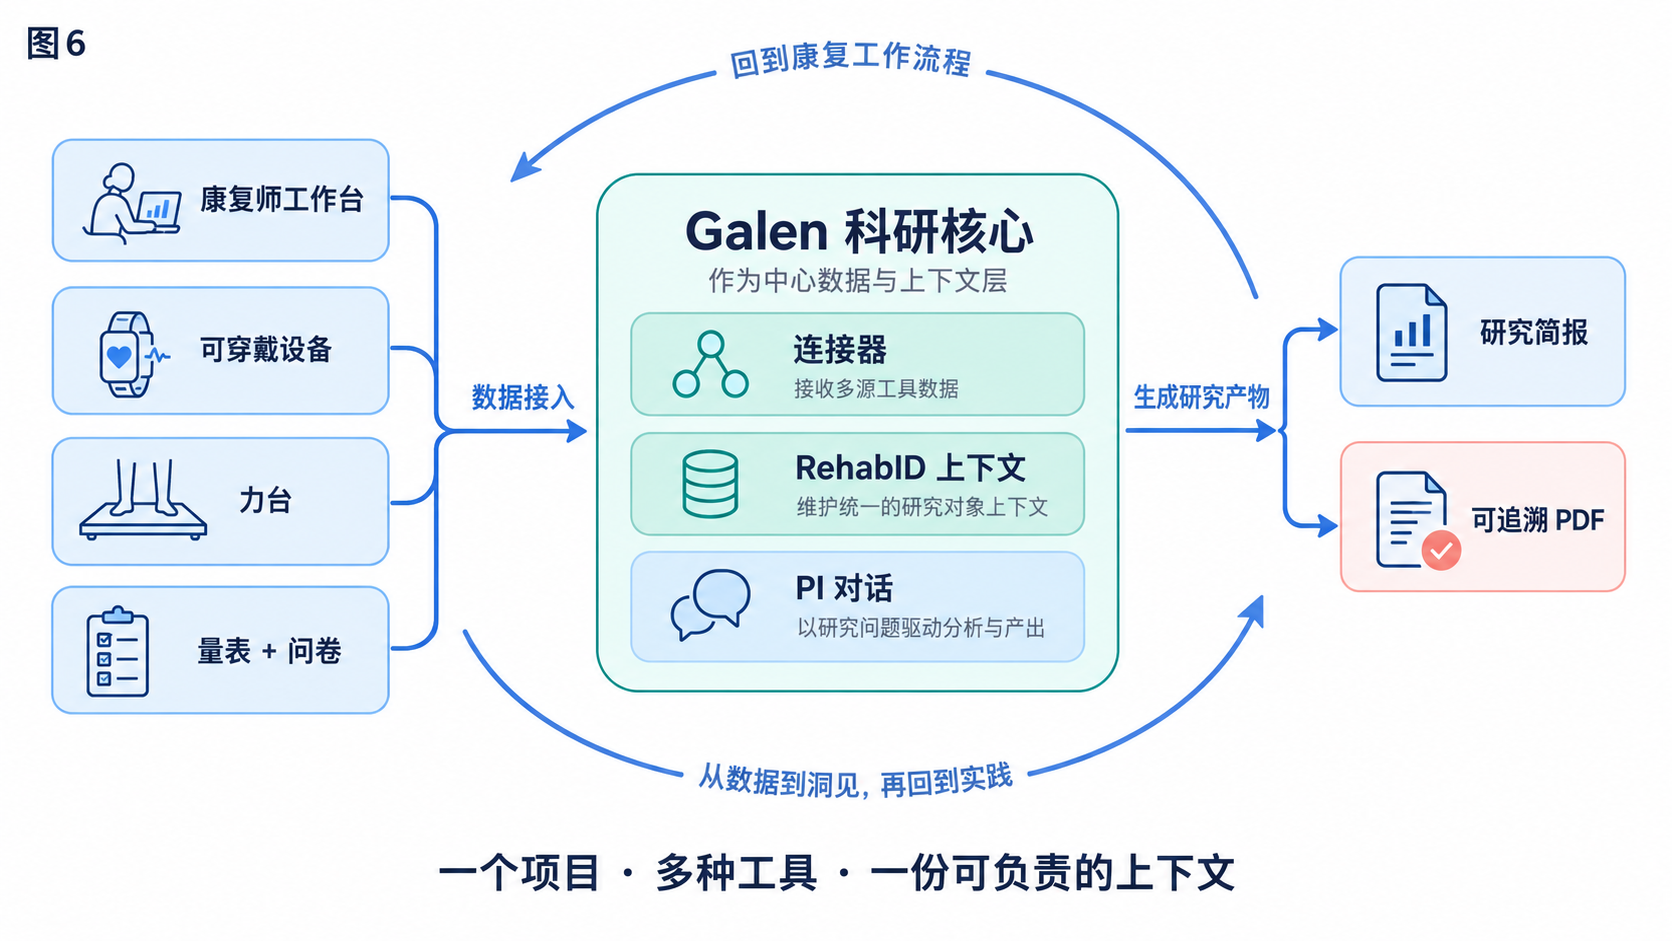
\includegraphics[width=0.98\linewidth]{assets/fig06-product-ecosystem-zh.png}
\caption*{产品与科研闭环：康复工具通过连接器进入 Galen，经过 RehabID 上下文与 PI 对话，返回研究产物和工作流程。}
\end{figure}

\clearpage
\section{从数据到正式论文的可见交付}
连接器导入完成后，Galen 以当前研究范围、RehabID 队列和任务节点驱动分析。产物不是聊天中的一段建议，而是可预览的正式论文 PDF；研究者可继续从论文预览回溯数据、证据和任务过程。

正式交付遵循“先事实、后解释、再结论”的顺序。事实层记录样本、时间点、变量和质量状态；解释层给出变化、对照和统计方法；结论层只引用已被数据或文献支持的内容。图表和表格不作为装饰，而是把关键中间结果暴露出来：读者可以从图表回到 RehabID 时间轴，从时间轴回到原始来源，再回到任务日志中的处理步骤。

\begin{figure}[htbp]
\centering
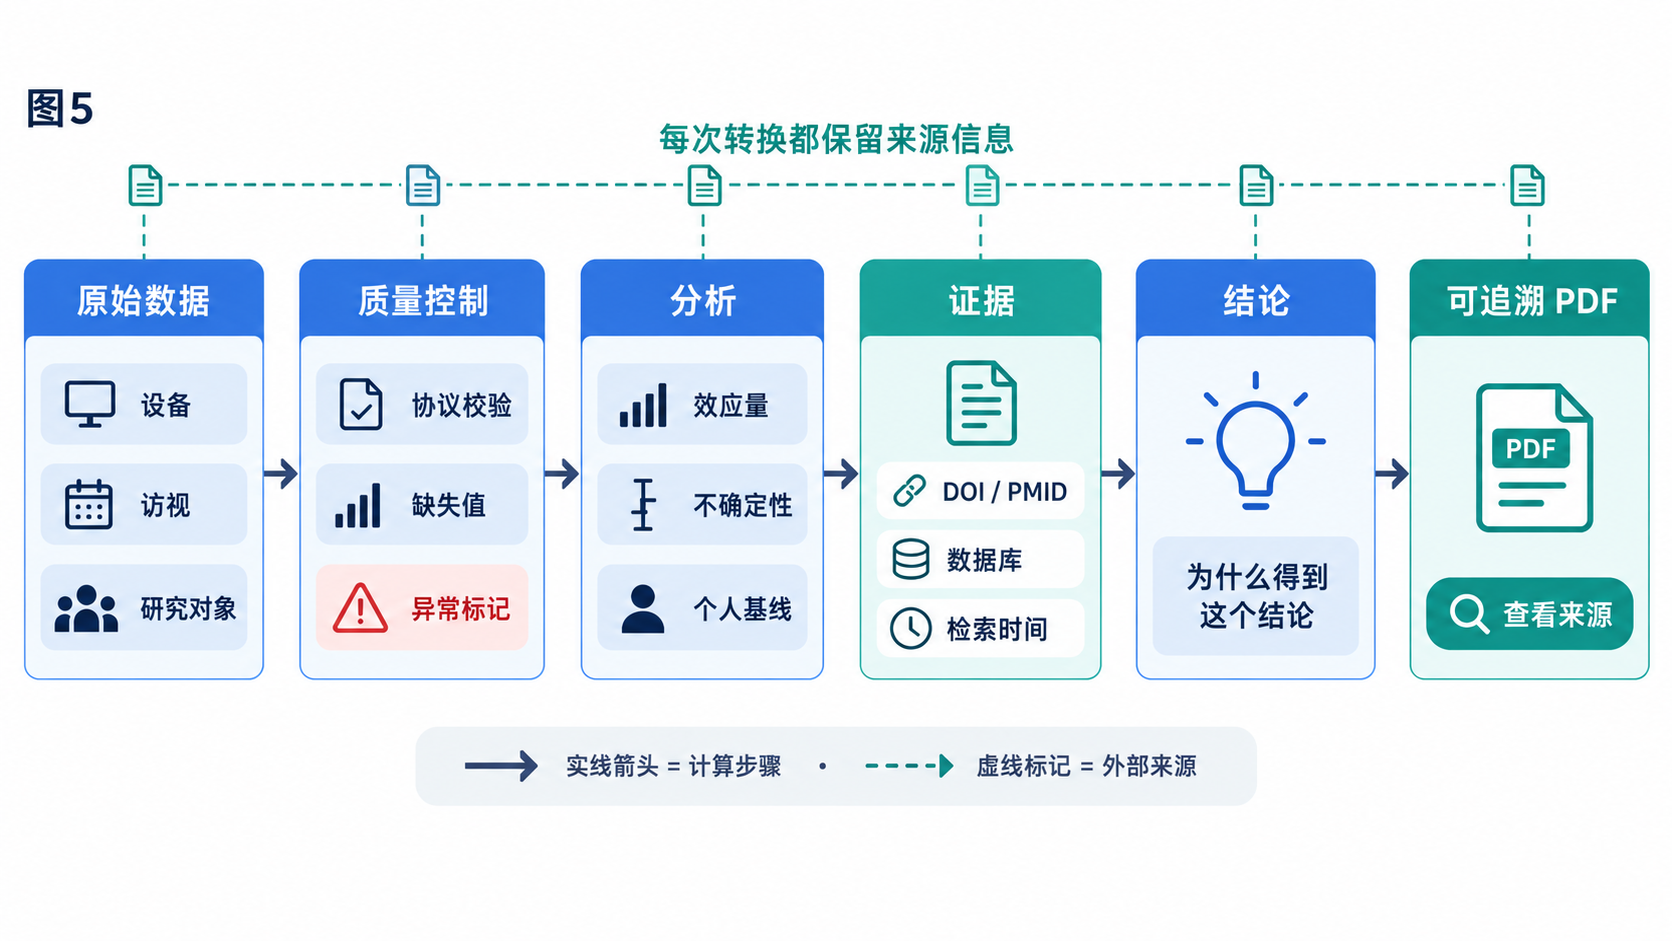
\includegraphics[width=0.98\linewidth]{assets/fig05-evidence-chain-zh.png}
\caption*{证据追溯链：从原始数据、质量控制和分析，到外部文献、研究结论与可追溯 PDF。}
\end{figure}

\begin{figure}[htbp]
\centering
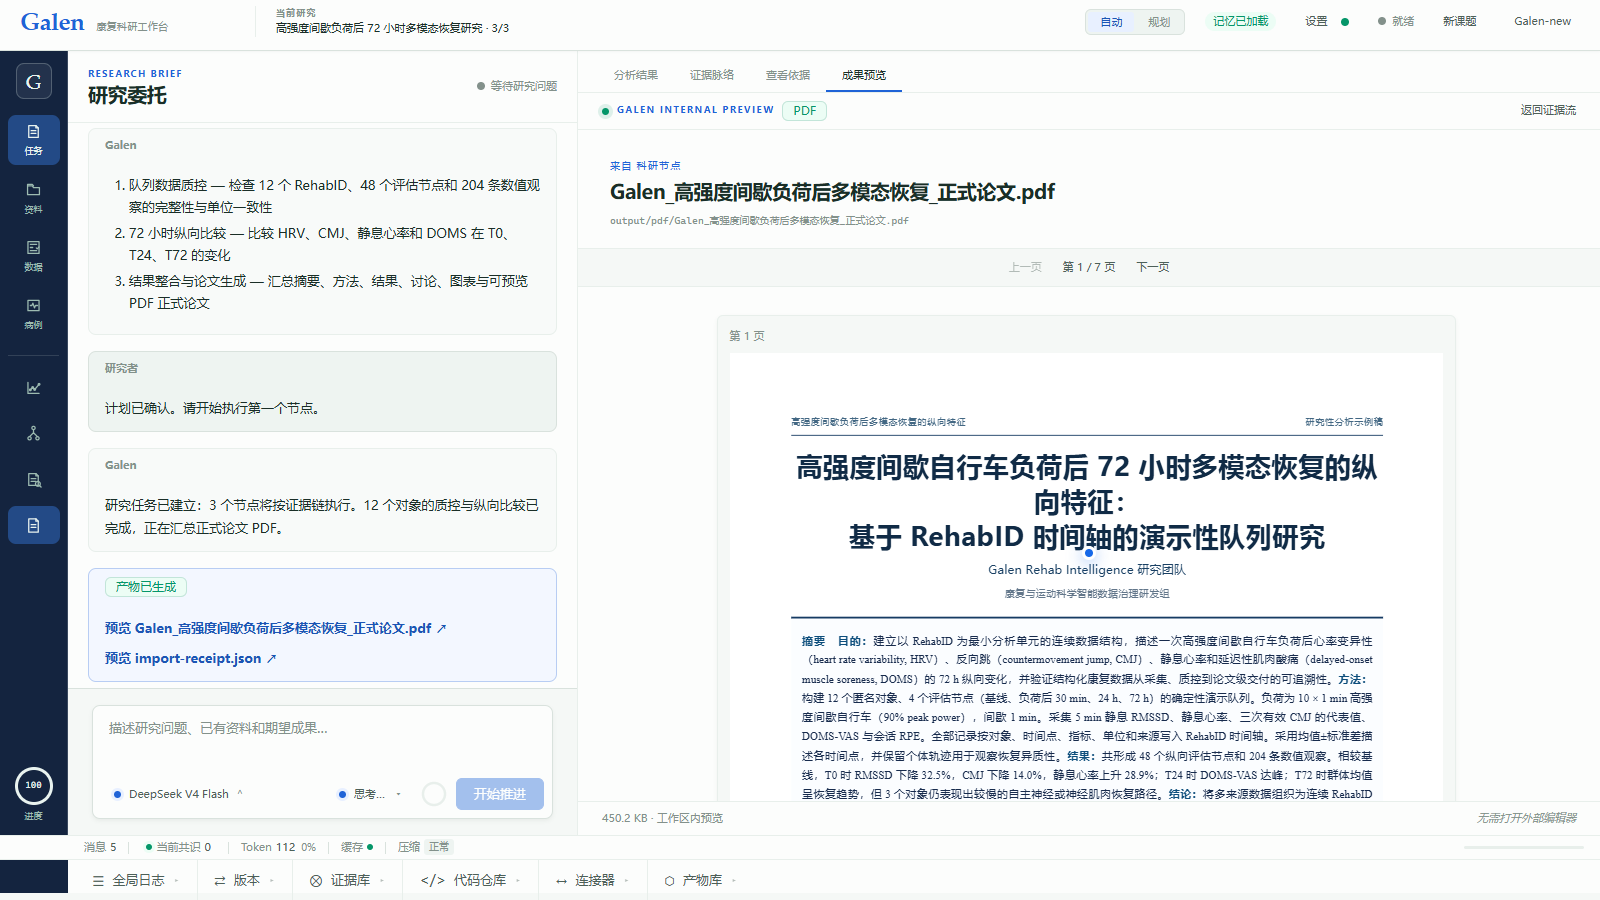
\includegraphics[width=0.94\linewidth]{assets/paper-preview.png}
\caption{Galen 交付的正式论文 PDF 全文预览，页面内保留研究任务与产物入口。}
\end{figure}

\begin{table}[H]
\centering
\small
\begin{tabularx}{\linewidth}{@{}p{3.4cm}Y p{3.0cm}@{}}
\toprule
论文中的对象 & 应能回到的来源 & 当前实现状态 \\
\midrule
样本与观察数 & RehabID 队列、访视记录、数据字典 & 已在连接器预览中展示 \\
质量控制结论 & 规范化日志、缺失/异常检查结果 & 数据契约已定义，逐条 QC 报告持续补齐 \\
变化图表 & 对齐后的纵向时间轴与分析脚本 & 已形成 PDF 图表和可复编译源文件 \\
文献判断 & 文献检索结果、文章标识、引用格式 & 检索/核验工具已接入，逐条主张审计为下一阶段 \\
最终段落 & 任务版本、模型调用和修订日志 & 机器可读 JSON 已保留 \\
\bottomrule
\end{tabularx}
\caption{论文对象与证据来源的对应关系。}
\end{table}

\section{代码与结果的可复核性}
\subsection{自动化测试}
Galen 上下文引擎的自动化测试覆盖记忆注入、长上下文压缩、任务状态迁移、工具调用边界、文献覆盖状态和论文 PDF 交付流程。本次本地执行结果为 \textbf{40/40 通过}。

\begin{center}
\fbox{\begin{minipage}{0.92\linewidth}
\ttfamily\small
> cargo test context\_tests --lib\\
running 40 tests\\
test context\_engine\_tests::memory\_long\_is\_indexed ... ok\\
test context\_engine\_tests::plan\_summary\_uses\_active\_task ... ok\\
test context\_engine\_tests::paper\_pdf\_delivery\_completes ... ok\\
test result: ok. 40 passed; 0 failed; 0 ignored
\end{minipage}}
\end{center}

\subsection{机器可读验证产物}
每次探针均输出 JSON 报告，其中保留模型名称、三轮提示、回答、工具轨迹、断言结果、会话消息数、令牌量和总耗时。本报告随源文件保留以下两份机器可读产物：
\begin{enumerate}[leftmargin=2em,itemsep=2pt]
\item \texttt{context-memory-probe.json}：连续约束修订，9/9 通过；
\item \texttt{fatigue-scope-probe.json}：运动疲劳范围切换，8/8 通过。
\end{enumerate}

\section{受控框架对照实验：验证架构而非“模型聪明度”}
前述探针证明 Galen 自己能跑通关键链路，但还不能回答“为什么要采用这套架构”。为此，项目另行完成了一份框架对照实验：把 Galen 与通用 CLI Agent 放在同一套冻结任务卡、同一模型标签和独立临时工作区中，比较它们完成康复科研任务的方式。该实验文档及原始运行记录已纳入本报告的证据包。

\subsection{实验问题与受控条件}
实验围绕三个问题展开：\textbf{（1）}在同一套任务卡上，项目状态是否提升硬门完成率；\textbf{（2）}显式的数据契约和工具边界是否减少无效调用与端到端时延；\textbf{（3）}失败是否集中在可以被架构定位的任务类型。任务卡分为上下文保持（PCTX01--05）、数据治理（PDATA01--05）和工具/交付（PTOOL01--05）三组，每张卡固定必需事实、必需产物、禁用事实、工具预算、最大模型请求次数和重复上限。

Galen 与 Codex CLI 均完成 15 张卡、每卡 5 次，共 75 次配对运行；两者使用同一 DeepSeek v4 Flash 配置和相同任务输入。OpenCode 完成 15 卡先导，并对上下文、数据、工具各选 1 张代表卡重复 5 次。Claude Code 只做单卡适配 smoke，不进入主统计。所有外部事件保守归一化，未暴露的 token、检索来源或工具事件不作推断。

\subsection{硬门与统计口径}
一次运行只有在进程完成、模型与工具未超预算、必需事实全部保留、产物存在且可预览、工具顺序满足约束、无重复调用环路且无禁用内容时才算通过。对通过率报告 Wilson 95\% 区间；Galen 与 Codex 在相同卡片和重复编号上配对，使用精确 McNemar 检验和固定种子的配对 bootstrap。这里的“通过”是工作流完成，不是临床效果或回答文采评分。

\begin{table}[H]
\centering
\small
\begin{tabularx}{\linewidth}{@{}p{4.1cm}cccY@{}}
\toprule
系统 & 覆盖 & 通过率 & 平均工具调用 & 中位总时延 \\
\midrule
Galen（完整架构） & 75 次 & 72/75（96.0\%） & 1.96 次 & 9.8 秒 \\
Codex CLI + DeepSeek & 75 次 & 17/75（22.7\%） & 11.64 次 & 32.2 秒 \\
OpenCode + DeepSeek（全套先导） & 15 次 & 9/15（60.0\%） & -- & -- \\
OpenCode + DeepSeek（代表卡重复） & 15 次 & 15/15（100\%） & -- & -- \\
\bottomrule
\end{tabularx}
\caption{冻结任务卡上的框架对照结果。OpenCode 的两种覆盖单独呈现，不与 75 次重复合并。}
\end{table}

\begin{figure}[H]
\centering
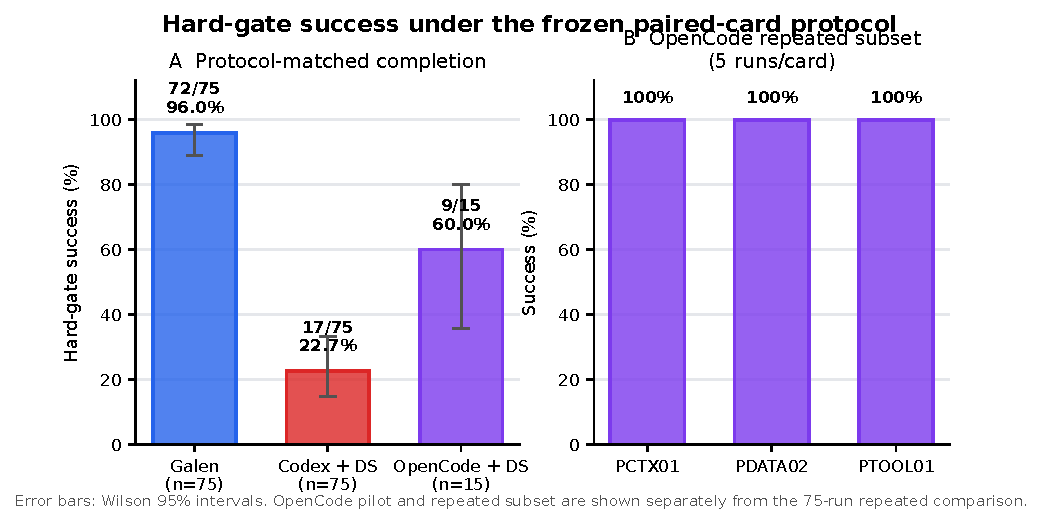
\includegraphics[width=0.96\linewidth]{assets/fig07-framework-success.pdf}
\caption{框架对照的硬门完成率。Galen 与 Codex 为 15 张卡、每卡 5 次；OpenCode 为先导和代表卡分层重复。}
\end{figure}

\begin{figure}[H]
\centering
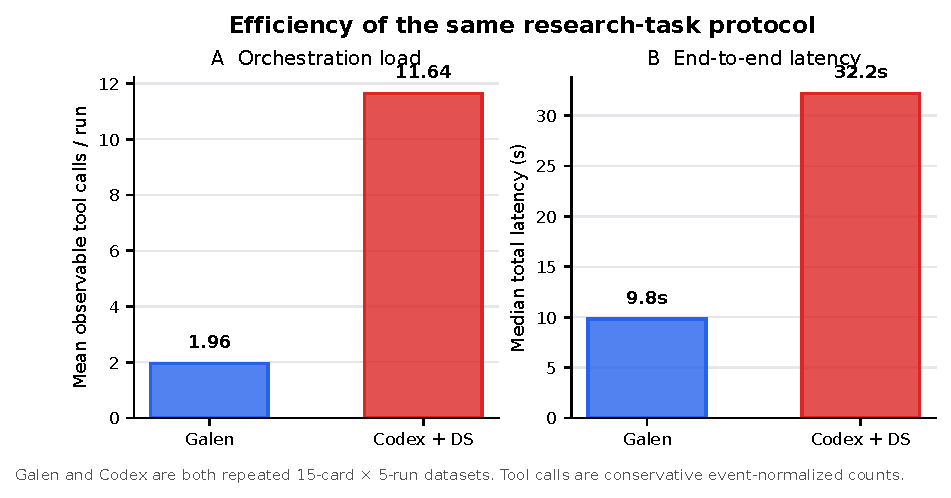
\includegraphics[width=0.96\linewidth]{assets/fig08-framework-efficiency.pdf}
\caption{工具调用与端到端时延。数值来自 Galen/Codex 的 75 次配对运行，工具调用按事件语义保守归一化。}
\end{figure}

\subsection{结果与解释}
在本协议定义的任务范围内，Galen 通过 72/75 次（96.0\%，Wilson 95\% CI：88.9--98.6\%），Codex 通过 17/75 次（22.7\%，CI：14.7--33.3\%）。配对结果为：双方同时通过 17 次，Galen 单独通过 55 次，Codex 单独通过 0 次，双方同时未通过 3 次；通过率差为 73.3 个百分点（配对 bootstrap 95\% CI：62.7--82.7），精确 McNemar $p<10^{-15}$。这组结果说明，在冻结任务卡和相同模型条件下，显式项目状态、数据契约、工具预算与产物验收组合起来，确实改变了科研任务的完成稳定性。

工具调用和时延也呈现一致方向：Galen 平均 1.96 次可观察工具调用、Codex 11.64 次；中位总时延分别为 9.8 秒和 32.2 秒。这里的含义不是“调用越少越好”，而是 Galen 更早把探索收敛到项目状态、必需事实和交付文件，减少了重复读取、目录探索和失败恢复带来的额外动作。

\begin{figure}[H]
\centering
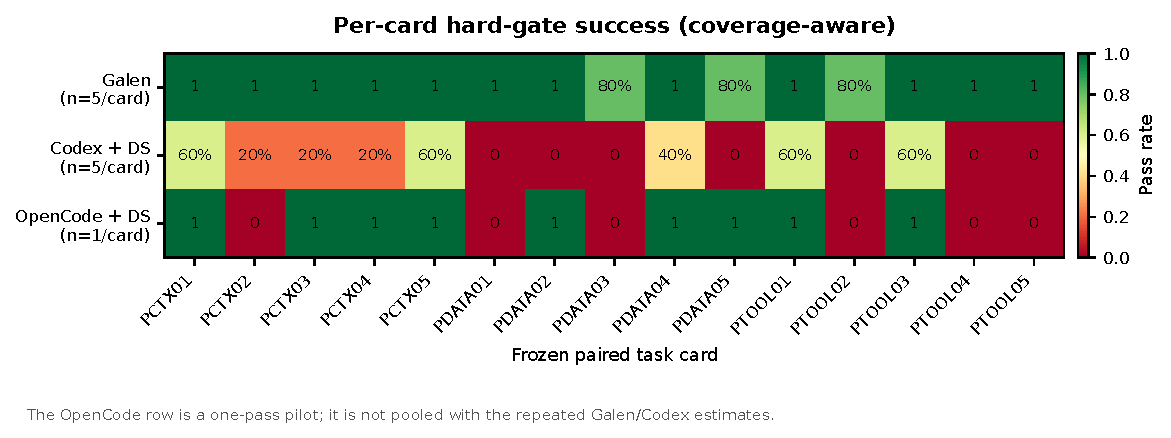
\includegraphics[width=0.98\linewidth]{assets/fig09-framework-failure.pdf}
\caption{按任务卡展示的失败边界。失败被定位到长上下文、数据时间对齐、工具恢复和交付检查等具体环节。}
\end{figure}

\subsection{这组实验能支持什么}
这不是“Galen 全面优于所有 Agent”的宣称。它支持的有限结论是：当任务同时要求持久项目状态、结构化数据治理、受控工具编排和可验证交付时，把这些约束写进执行架构，比直接把通用 CLI 当作科研工作台更稳定、更经济。实验还暴露了 Galen 自身的失败卡（PDATA01、PTOOL02、PDATA05），以及外部框架在长上下文、时间对齐和工具恢复上的边界；这些失败记录将直接进入下一轮修复，而不是从结果中删除。

\subsection{实验材料}
对照实验的完整材料和先导摘要均在项目目录中保留：
\begin{itemize}[leftmargin=2em,itemsep=1pt]
\item 完整报告：\path{output/pdf/galen-framework-comparison/}\\
\path{galen_framework_comparison_report.pdf}
\item 先导摘要：\path{evals/runs/}\\
\path{framework-comparison-pilot-20260912-summary.md}
\end{itemize}
任务协议、运行 JSONL、原始事件和图表脚本也在实验目录中保留，可据此复跑或扩展到更多框架。

\section{人工判读对照的实施方式}
为完成用户应用结果与人工判断的一致性对比，后续由 3 名具有康复科研训练的评阅者对同一组三轮任务进行独立判读。评阅者不查看系统断言，按表 \ref{tab:human-rubric} 对最终方案评分；系统输出与人工判读将按项目逐项对齐，形成一致率与分歧案例表。

\begin{table}[htbp]
\centering
\small
\begin{tabularx}{\linewidth}{@{}p{3.2cm}Yc@{}}
\toprule
人工判读维度 & 判断标准 & 得分 \\
\midrule
当前范围遵循 & 是否仅使用当前研究方向、对象、变量与观察窗 & 0 / 1 / 2 \\
核心事实保留 & 协议、样本、时点、变量与数据字典是否完整 & 0 / 1 / 2 \\
归档范围隔离 & 已归档方向是否未进入新方案正文与最终回答 & 0 / 1 / 2 \\
交付可用性 & 方案是否可直接作为下一步分析的输入 & 0 / 1 / 2 \\
\bottomrule
\end{tabularx}
\caption{人工判读量表。0 为不满足，1 为部分满足，2 为完全满足。}
\label{tab:human-rubric}
\end{table}

\section{结果解读：本轮已经证明什么}
本轮结果可以支持三个明确判断。第一，Galen 能在同一项目中保留跨轮次的协议、样本、结局和工具事实，并把随访从 12 周修订为 16 周；这证明状态更新不是简单追加聊天文本。第二，Galen 能把已归档方向与当前运动疲劳范围分开，8 项范围断言全部通过；这证明项目切换有可执行的隔离规则。第三，连接器、RehabID、分析任务和 PDF 交付已经在一条可观看、可复跑的流程中连通；这证明系统具备从数据进入到研究产物的最小闭环。

这些结果还不能支持另外三个更强的判断：不能据此声称 Galen 的临床判断优于医生，不能据此声称其检索覆盖率优于所有数据库，也不能据此声称其在不同模型、不同机构和不同设备上已经稳定。后续对照实验会使用固定任务卡和统一数据，报告基线系统与 Galen 的差异，并把失败案例而不是只把通过案例纳入分析。

\section{当前缺口与下一阶段验收}
\begin{enumerate}[leftmargin=2.1em,itemsep=4pt]
\item \textbf{主张级引用审计：}为论文中的每条科研建议生成唯一来源指针，区分原始数据、外部文献和模型推断，并统计证据覆盖率 $C$；
\item \textbf{数据质量报告：}将缺失、重复、单位冲突、时间异常和异常值检查固化为可下载的 QC 产物，避免只在界面中显示“已处理”；
\item \textbf{受控基线比较：}在同一模型、同一任务和同一数据下，对比无项目状态的聊天流程、传统 RAG 流程与 Galen，报告约束保留、范围隔离、产物完成和令牌开销；
\item \textbf{人工一致性验证：}由至少 3 名具有康复科研训练的评阅者按表 \ref{tab:human-rubric} 独立复核，并记录分歧案例；
\item \textbf{跨来源扩展：}在现有康复师工作台之外，逐步接入力台、可穿戴、量表和传感器数据，先验证数据契约，再决定是否自研硬件。
\end{enumerate}

上述缺口是下一轮可执行的验收项，不是对当前结果的否定。它们把“系统已经能跑通”推进为“系统在可比较、可审计的条件下值得信任”。

\section{结论}
现有验证表明，Galen 已具备将研究项目约束、范围修订、工具读取事实与 RehabID 数据队列连接至同一科研工作流的能力。它的技术主张可以被压缩为一句话：\textbf{让康复科研数据在正确的项目状态中被接入、清洗、对齐、解释、引用并交付。}两组真实模型探针、40/40 自动化测试、连接器流程和正式 PDF 共同构成了这条主张的第一组证据。

Galen 的价值在于固定数据来源、项目范围和证据回链；补齐主张级引用、质量产物与受控基线后，它将成为可复用的康复科研数据治理基础设施。

\end{document}
